\section{Customizing Stable Diffusion}
\begin{frame}[plain]
    \centering
    \vspace{2cm}
    {\Huge \textcolor{blue}{Stable Diffusion:}\\[1em]
     \textbf{Customizing Stable Diffusion}}
\end{frame}

\begin{frame}{Personalization: Textual Inversion, DreamBooth, LoRA}
  \begin{itemize}\itemsep0.3em
    \item Open weights made SD the platform people \textbf{fine-tune}; three techniques cover most of it:
    \item \textbf{Textual Inversion} (Gal et al., 2023): learn a \textbf{new token embedding} for a concept from a few images; the rest of the model stays frozen ($\sim$kilobytes per concept).
    \item \textbf{DreamBooth} (Ruiz et al., 2023): fine-tune the model itself to bind a \textbf{rare token} to a specific subject (your pet, a product), with a prior-preservation loss against forgetting the class.
    \item \textbf{LoRA} (Hu et al., 2022): train \textbf{low-rank adapters} on the attention weights instead of the full model; megabytes instead of gigabytes, composable, and cheap to share. The de facto standard for style and character adaptation.
  \end{itemize}
\end{frame}

\begin{frame}[allowframebreaks]{DreamBooth}
\begin{figure}
    \centering
    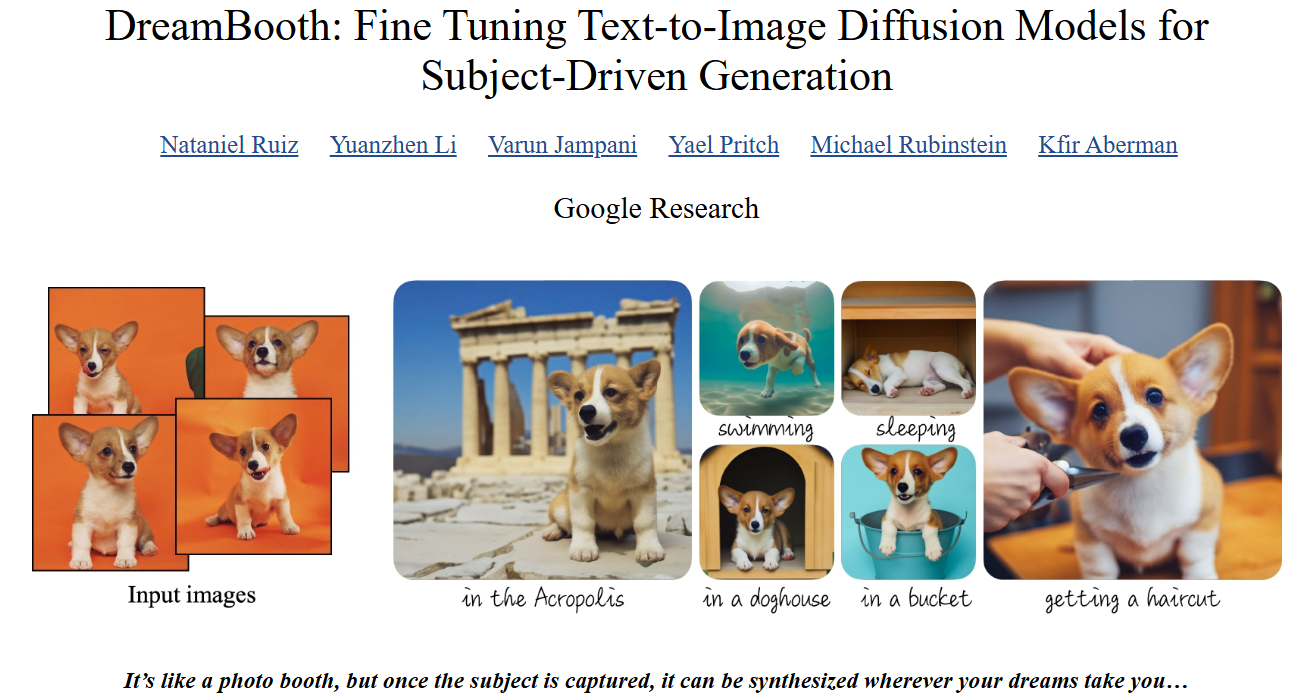
\includegraphics[width=0.5\linewidth,height=0.5\textheight,keepaspectratio]{images/adv-img-gen/dreambooth-1.png}
    \caption*{\scriptsize Source: Ruiz et al., \href{https://arxiv.org/abs/2208.12242}{``DreamBooth''}, CVPR 2023.}
\end{figure}

\framebreak
\textbf{What is DreamBooth?}
\begin{itemize}
    \item A method for fine-tuning large diffusion models on a small number of images.
    \item Developed by Google Research; published at CVPR 2023.
    \item Allows personalization of generative models with minimal data.
\end{itemize}

\framebreak
\textbf{Key Concepts}
\begin{itemize}
    \item \textbf{Personalization:} Adapts a pre-trained model to generate images of specific subjects (e.g., pets, people).
    \item \textbf{Fine-tuning:} Uses a small set of images to adjust the model's parameters.
    \item \textbf{Text Conditioning:} Uses text prompts to guide image generation.
\end{itemize}

\framebreak

\begin{figure}
    \centering
    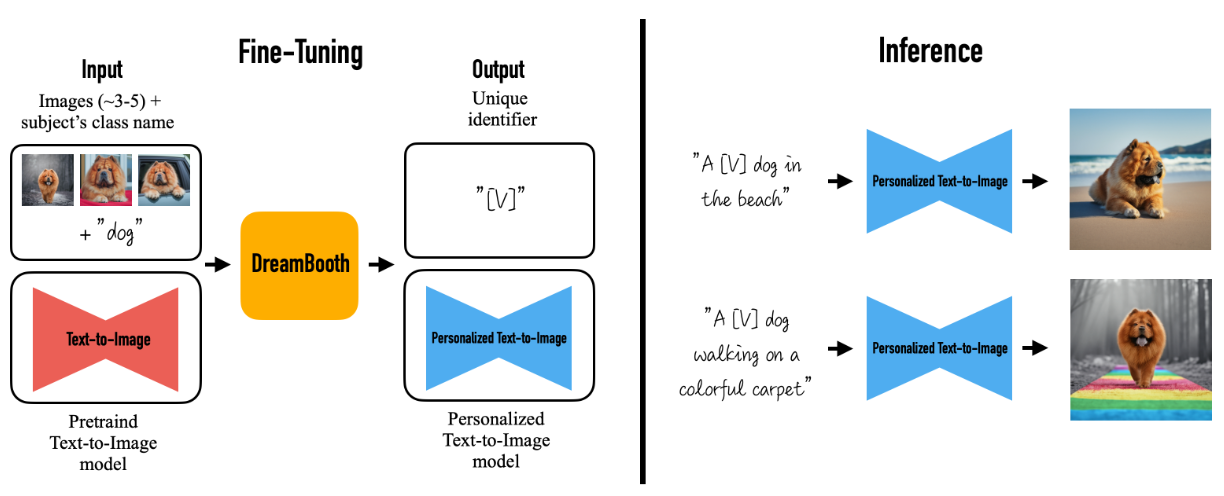
\includegraphics[width=\linewidth,height=0.78\textheight,keepaspectratio]{images/adv-img-gen/dreambooth-2.png}
    \caption*{\scriptsize Source: Ruiz et al., \href{https://arxiv.org/abs/2208.12242}{``DreamBooth''}, CVPR 2023.}
\end{figure}

\framebreak

\textbf{How Does DreamBooth Personalize Models?}
\begin{itemize}
    \item DreamBooth teaches a model to recognize a new subject using just a few photos.
    \item After training, the model can create new images of that subject in different places or situations.
    \item This is called ``few-shot'' learning: only a few examples are needed.
\end{itemize}

\framebreak
\begin{figure}
    \centering
    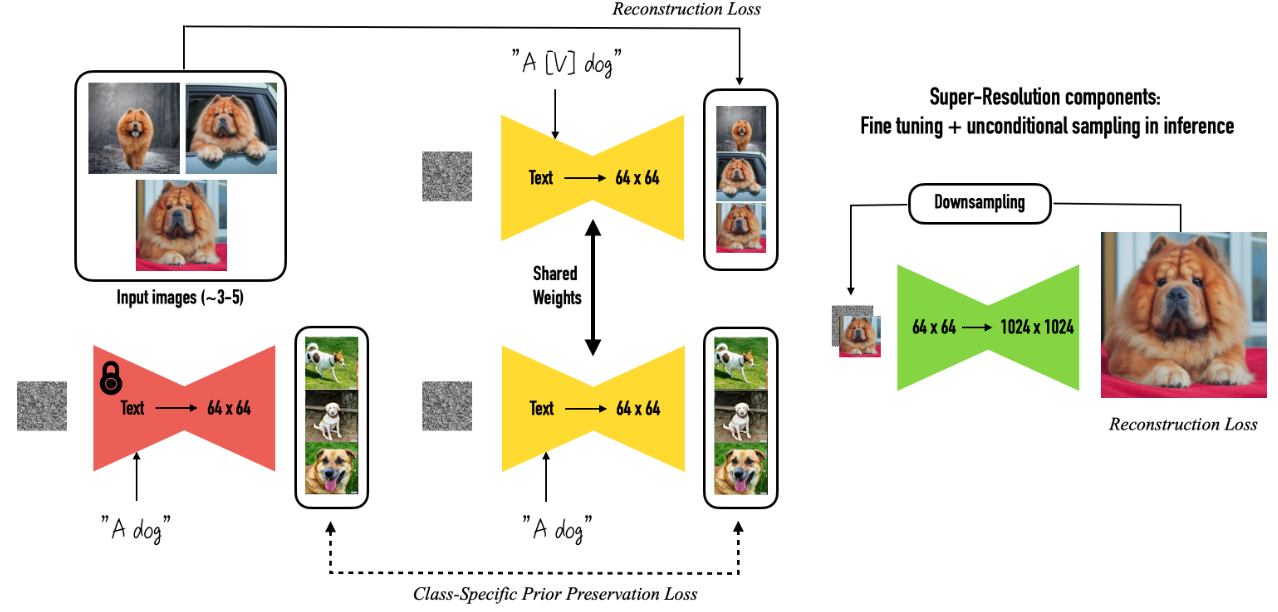
\includegraphics[width=\linewidth,height=0.78\textheight,keepaspectratio]{images/adv-img-gen/dreambooth-3.png}
    \caption*{\scriptsize Source: Ruiz et al., \href{https://arxiv.org/abs/2208.12242}{``DreamBooth''}, CVPR 2023.}
\end{figure}

\framebreak

\textbf{How Do We Tell the Model About the New Subject?}
\begin{itemize}
    \item We bind the subject to a \textit{rare token}: an existing vocabulary token that the model has almost never seen in training.
    \item For example: ``a photo of \texttt{sks dog} at the beach'' (\texttt{sks} is the community convention popularised by the \texttt{diffusers} examples, not a token from the paper).
    \item The model learns to link this rare-token to the subject in your photos.
\end{itemize}

\framebreak

\textbf{Why Use Rare-tokens?}
\begin{itemize}
    \item Rare tokens are existing vocabulary tokens that appear very infrequently, so they carry a weak prior and are easy to rebind.
    \item This avoids mixing up your subject with things the model already knows.
\end{itemize}

\framebreak

\textbf{How Does DreamBooth Avoid Forgetting?}
\begin{itemize}
    \item If we only train on your subject, the model might forget how to make other images.
    \item To prevent this, we also show it regular class prompts (like ``a photo of a dog'').
    \item We use a special loss to balance learning the new subject and keeping old knowledge:
    \[
        \mathcal{L}_{\text{total}} = \mathcal{L}_{\text{subject}} + \lambda \mathcal{L}_{\text{prior}}
    \]
    where:
    \begin{itemize}
        \item $\mathcal{L}_{\text{subject}}$ = loss for your subject (rare-token prompt)
        \item $\mathcal{L}_{\text{prior}}$ = loss for general class (class prompt)
        \item $\lambda$ = weight to balance the two
    \end{itemize}
\end{itemize}
\end{frame}

\begin{frame}[allowframebreaks]{DreamBooth: Results}
\begin{figure}
    \centering
    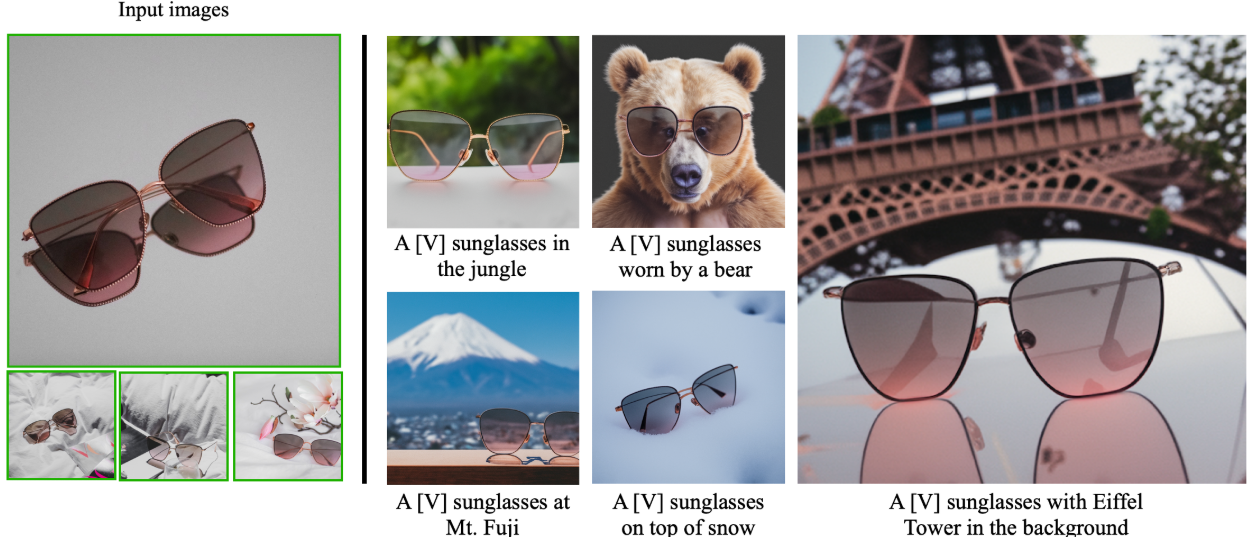
\includegraphics[width=\linewidth,height=0.78\textheight,keepaspectratio]{images/adv-img-gen/dreambooth-result-1.png}
    \caption*{\scriptsize Source: Ruiz et al., \href{https://arxiv.org/abs/2208.12242}{``DreamBooth''}, CVPR 2023.}
\end{figure}

\framebreak

\begin{figure}
    \centering
    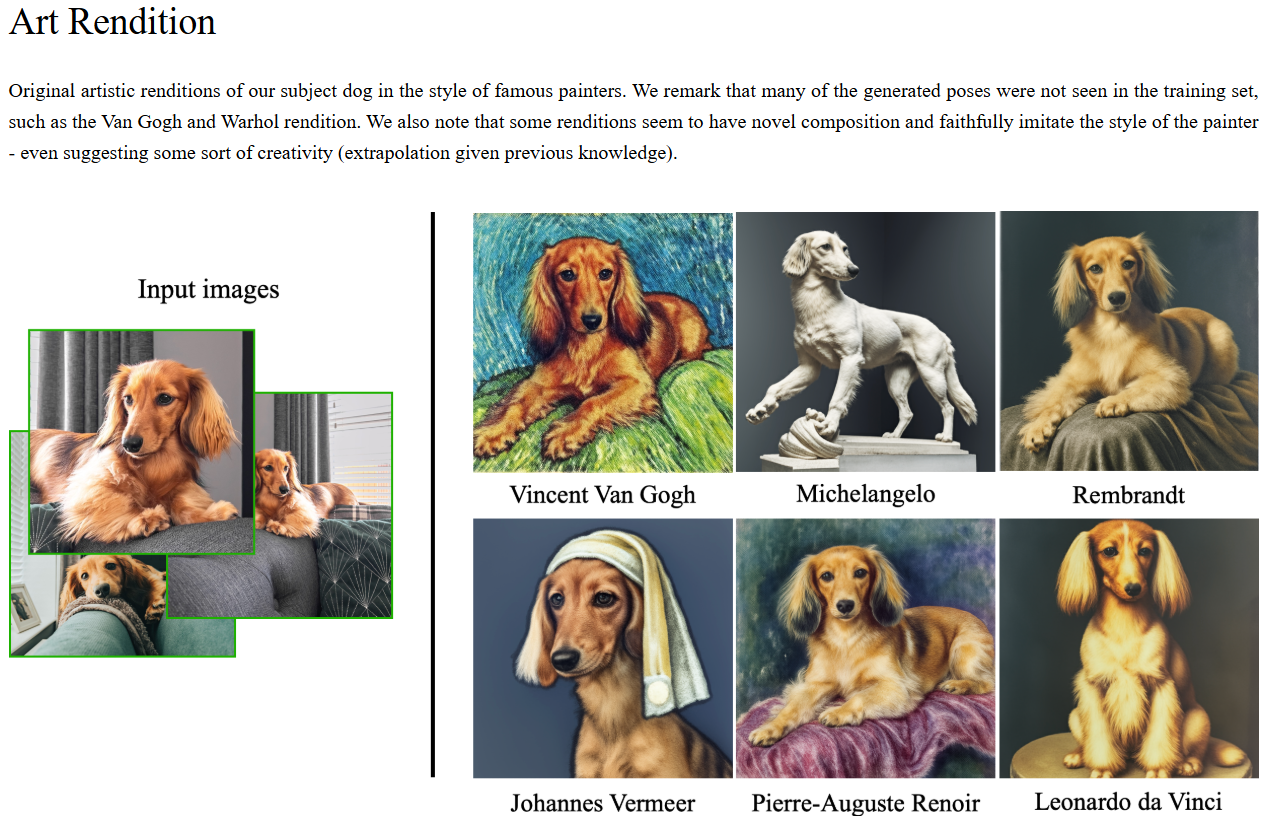
\includegraphics[width=\linewidth,height=0.78\textheight,keepaspectratio]{images/adv-img-gen/dreambooth-result-2.png}
    \caption*{\scriptsize Source: Ruiz et al., \href{https://arxiv.org/abs/2208.12242}{``DreamBooth''}, CVPR 2023.}
\end{figure}

\framebreak
\begin{figure}
    \centering
    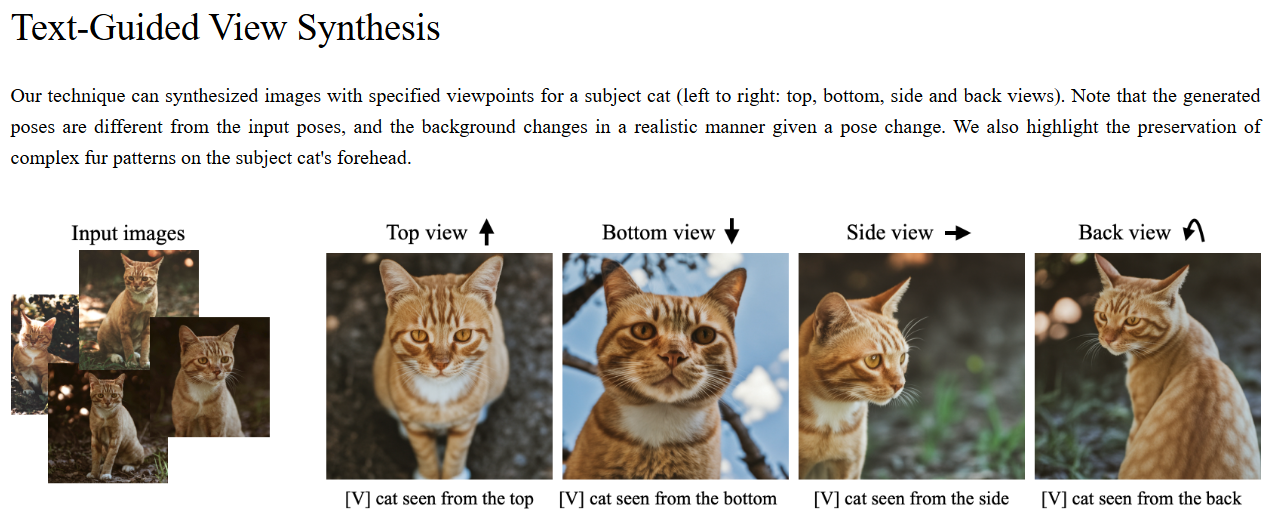
\includegraphics[width=\linewidth,height=0.78\textheight,keepaspectratio]{images/adv-img-gen/dreambooth-result-3.png}
    \caption*{\scriptsize Source: Ruiz et al., \href{https://arxiv.org/abs/2208.12242}{``DreamBooth''}, CVPR 2023.}
\end{figure}

\framebreak
\begin{figure}
    \centering
    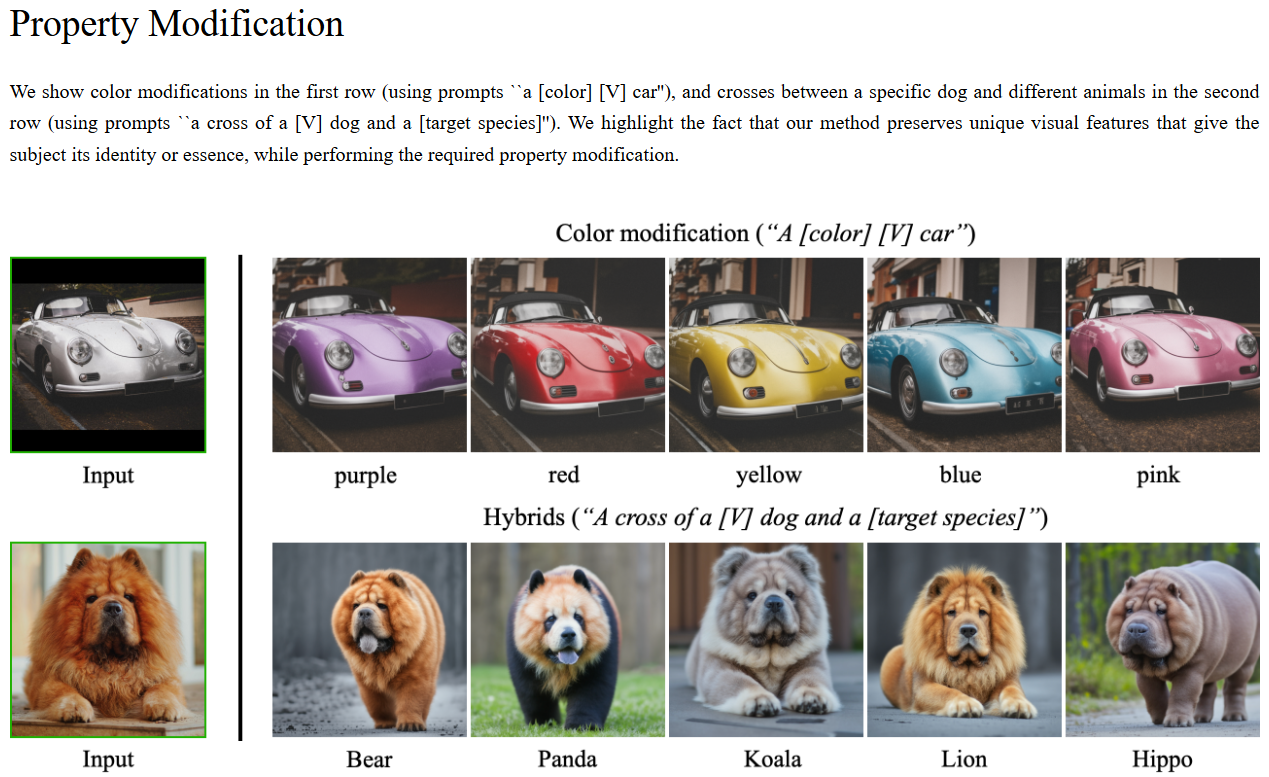
\includegraphics[width=\linewidth,height=0.78\textheight,keepaspectratio]{images/adv-img-gen/dreambooth-result-4.png}
    \caption*{\scriptsize Source: Ruiz et al., \href{https://arxiv.org/abs/2208.12242}{``DreamBooth''}, CVPR 2023.}
\end{figure}

\framebreak
\begin{figure}
    \centering
    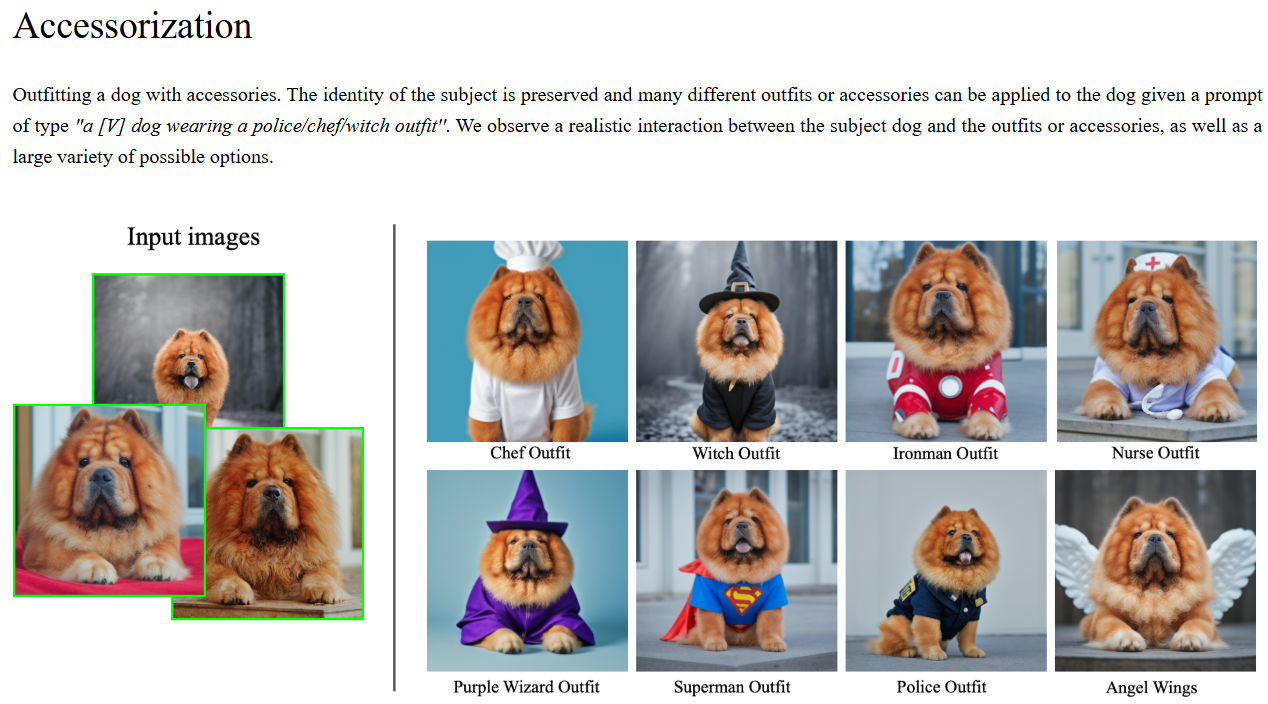
\includegraphics[width=\linewidth,height=0.78\textheight,keepaspectratio]{images/adv-img-gen/dreambooth-result-5.png}
    \caption*{\scriptsize Source: Ruiz et al., \href{https://arxiv.org/abs/2208.12242}{``DreamBooth''}, CVPR 2023.}
\end{figure}
\end{frame}
\begin{frame}[allowframebreaks]{Low-Rank Adaptation (LoRA)}
\begin{figure}
    \centering
    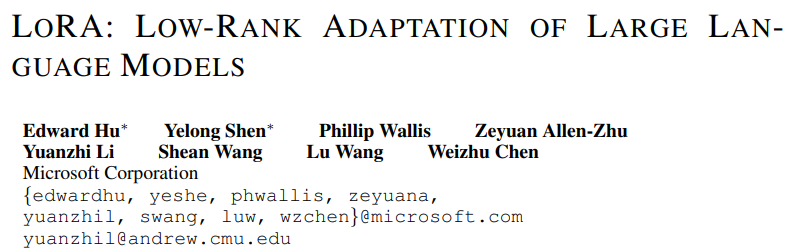
\includegraphics[width=\linewidth,height=0.72\textheight,keepaspectratio]{images/adv-img-gen/lora-1.png}
    \caption*{\scriptsize Source: Hu et al., \href{https://arxiv.org/abs/2106.09685}{``LoRA: Low-Rank Adaptation of Large Language Models''}, ICLR 2022.}
\end{figure}

\framebreak

\large \textbf{LoRA Overview}\\[0.5ex]
Low-Rank Adaptation (LoRA) is a technique for efficient fine-tuning of large neural networks. Instead of updating all parameters, LoRA injects trainable low-rank matrices into each layer, significantly reducing the number of trainable parameters.

\textbf{Key Idea:} Decompose the weight update $\Delta W$ as a product of two low-rank matrices:
\begin{equation}
    \Delta W = B A
\end{equation}
where $B \in \mathbb{R}^{d \times r}$ and $A \in \mathbb{R}^{r \times k}$, with $r \ll \min(d, k)$. Following Hu et al., $A$ is the down-projection (random Gaussian init) and $B$ the up-projection (initialised to zero), so $\Delta W = 0$ at the start of training.

\framebreak

\begin{figure}
    \centering
    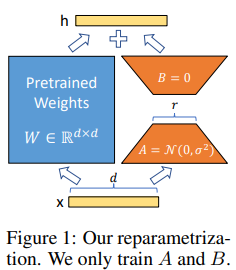
\includegraphics[width=\linewidth,height=0.72\textheight,keepaspectratio]{images/adv-img-gen/lora-2.png}
    \caption*{\scriptsize Source: Hu et al., \href{https://arxiv.org/abs/2106.09685}{``LoRA: Low-Rank Adaptation of Large Language Models''}, ICLR 2022.}
\end{figure}

\framebreak

\large \textbf{LoRA in Linear Layers}\\[0.5ex]
Consider a linear layer with weight $W_0 \in \mathbb{R}^{d \times k}$. In LoRA, the forward pass is modified as:
\begin{equation}
    y = W_0 x + \frac{\alpha}{r} B A x
\end{equation}
where $\alpha$ is a constant scaling factor and only $A$ and $B$ are updated during fine-tuning. Dividing by $r$ keeps the size of the update roughly independent of the rank, so $r$ can be changed without retuning the learning rate.

\textbf{Parameter Efficiency:} The number of trainable parameters is reduced from $d \times k$ to $r \times (d + k)$.

\framebreak
\large \textbf{LoRA Training Objective}\\[0.5ex]
The training objective remains the same as standard fine-tuning, e.g., minimizing a loss function $\mathcal{L}$:
\begin{equation}
    \min_{A, B} \mathcal{L}(\hat{y}, y)
\end{equation}
where $\hat{y}$ is the model output and $y$ is the ground truth.

\textbf{Regularization:} The rank bound is structural, not a penalty: $\Delta W = BA$ has rank at most $r$ by construction. Weight decay or dropout on the adapter branch can still be added to limit overfitting.

\framebreak
\large \textbf{LoRA in Attention Mechanisms}\\[0.5ex]
LoRA is commonly applied to the query and value projection matrices in attention layers:
\begin{align}
    W_q' &= W_q + \Delta W_q = W_q + \tfrac{\alpha}{r} B_q A_q \\
    W_v' &= W_v + \Delta W_v = W_v + \tfrac{\alpha}{r} B_v A_v
\end{align}
where $B_q, A_q, B_v, A_v$ are the low-rank factors for the query and value projections, respectively.

\framebreak

\begin{figure}
    \centering
    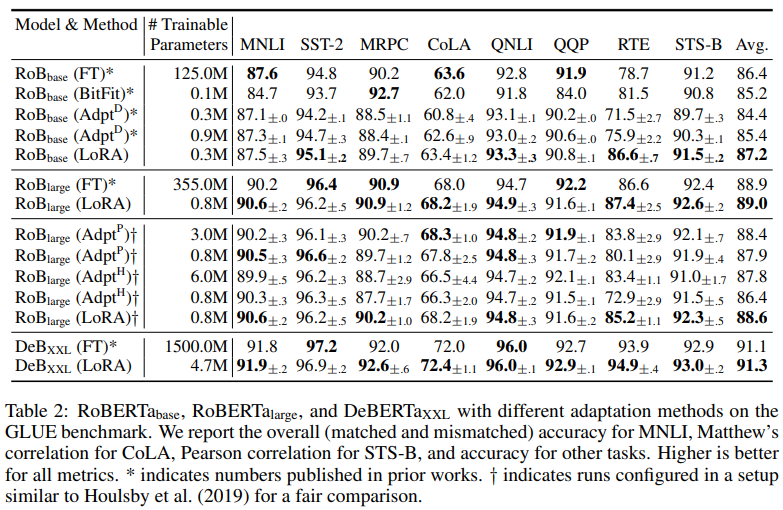
\includegraphics[width=\linewidth,height=0.72\textheight,keepaspectratio]{images/adv-img-gen/lora-3.png}
    \caption*{\scriptsize Source: Hu et al., \href{https://arxiv.org/abs/2106.09685}{``LoRA: Low-Rank Adaptation of Large Language Models''}, ICLR 2022.}
\end{figure}

\framebreak

\begin{figure}
    \centering
    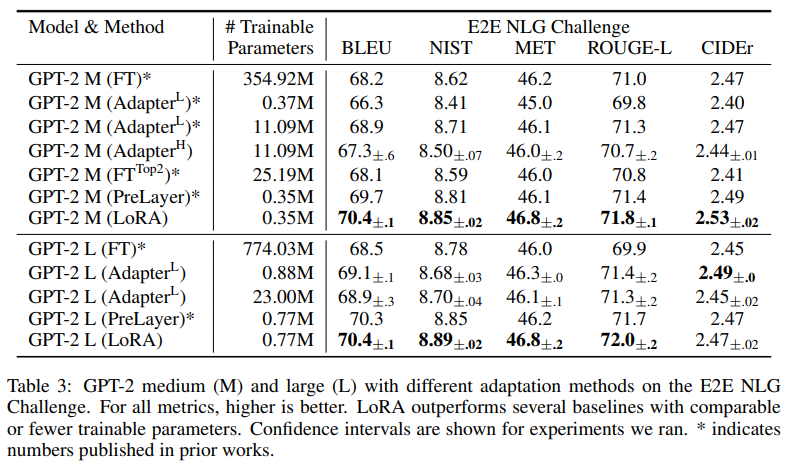
\includegraphics[width=\linewidth,height=0.72\textheight,keepaspectratio]{images/adv-img-gen/lora-4.png}
    \caption*{\scriptsize Source: Hu et al., \href{https://arxiv.org/abs/2106.09685}{``LoRA: Low-Rank Adaptation of Large Language Models''}, ICLR 2022.}
\end{figure}
\framebreak

\begin{figure}
    \centering
    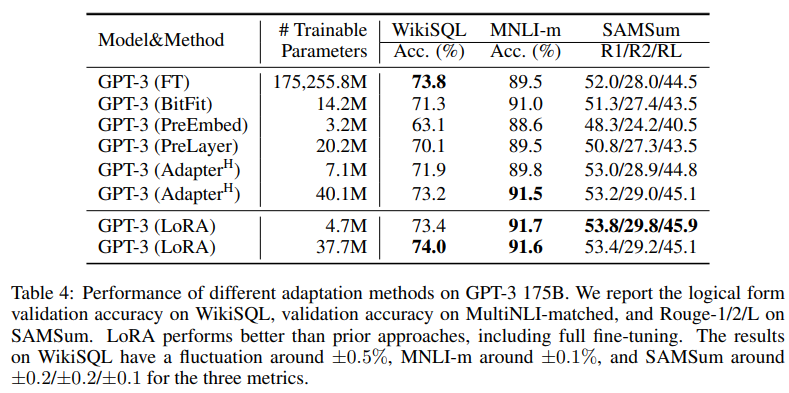
\includegraphics[width=\linewidth,height=0.72\textheight,keepaspectratio]{images/adv-img-gen/lora-5.png}
    \caption*{\scriptsize Source: Hu et al., \href{https://arxiv.org/abs/2106.09685}{``LoRA: Low-Rank Adaptation of Large Language Models''}, ICLR 2022.}
\end{figure}

\framebreak

\begin{figure}
    \centering
    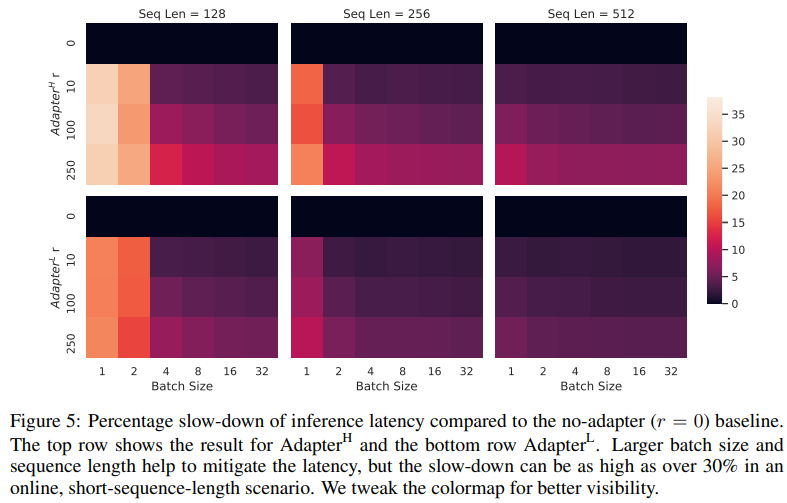
\includegraphics[width=\linewidth,height=0.72\textheight,keepaspectratio]{images/adv-img-gen/lora-6.png}
    \caption*{\scriptsize Source: Hu et al., \href{https://arxiv.org/abs/2106.09685}{``LoRA: Low-Rank Adaptation of Large Language Models''}, ICLR 2022.}
\end{figure}
\end{frame}

\begin{frame}{Spatial Control: ControlNet}
  \begin{itemize}\itemsep0.3em
    \item Text describes \emph{what}; it is poor at \emph{where}. \textbf{ControlNet} (Zhang et al., 2023) adds spatial conditioning: edge maps, human pose, depth, sketches, segmentation.
    \item Mechanism: clone the U-Net encoder into a \textbf{trainable copy} that ingests the condition image, keep the original weights \textbf{frozen}, and connect the copy through \textbf{zero-initialized convolutions} so training starts from a no-op and cannot damage the base model.
    \item Result: precise layout control with modest paired data, reusing everything the base model knows.
    \item Together with LoRA and inpainting, this is why an open 2022 model still anchors production pipelines today.
  \end{itemize}
\end{frame}
